\documentclass[a4paper,12pt]{article}
\usepackage{amsmath,amssymb,amsfonts,amsthm}
\usepackage{tikz}
\usepackage [utf8x] {inputenc}
\usepackage [T2A] {fontenc} 
\usepackage[russian]{babel}
\usepackage{cmap} 
\usepackage{ gensymb }
% Так ссылки в PDF будут активны
\usepackage[unicode]{hyperref}
\usepackage{ textcomp }
\usepackage{indentfirst}
\usepackage[version=3]{mhchem}

% вы сможете вставлять картинки командой \includegraphics[width=0.7\textwidth]{ИМЯ ФАЙЛА}
% получается подключать, как минимум, файлы .pdf, .jpg, .png.
\usepackage{graphicx}
% Если вы хотите явно указать поля:
\usepackage[margin=1in]{geometry}
% Или если вы хотите задать поля менее явно (чем больше DIV, тем больше места под текст):
% \usepackage[DIV=10]{typearea}

\usepackage{fancyhdr}

\newcommand{\bbR}{\mathbb R}%теперь вместо длинной команды \mathbb R (множество вещественных чисел) можно писать короткую запись \bbR. Вместо \bbR вы можете вписать любую строчку букв, которая начинается с '\'.
\newcommand{\eps}{\varepsilon}
\newcommand{\bbN}{\mathbb N}
\newcommand{\dif}{\mathrm{d}}

\newtheorem{Def}{Определение}


\pagestyle{fancy}
\makeatletter % сделать "@" "буквой", а не "спецсимволом" - можно использовать "служебные" команды, содержащие @ в названии
\fancyhead[R]{\footnotesize ФУПМ МФТИ}
\fancyfoot[L]{\footnotesize \@author}%имя автора будет написано внизу страницы слева
\fancyfoot[R]{\thepage}%номер страницы —- внизу справа
\fancyfoot[C]{}%по центру внизу страницы пусто

\renewcommand{\maketitle}{%
	\noindent{\bfseries\scshape\large\@title\ \mdseries\upshape}\par
	\noindent {\large\itshape\@author}
	\vskip 2ex}
\makeatother
\def\dd#1#2{\frac{\partial#1}{\partial#2}}


\title{4.1 \\ Определение энергии $\alpha$-частиц по величине их пробега в воздухе}
\author{Северилов Павел 674} 
\date{12 ноября 2018 г.}

\begin{document}
	
	\maketitle
	\section{Теоретическое введение}
		Энергию альфа-частиц удобно определять по величине их пробега в веществе. Рассмотрим подробно взаимодействие заряженных частиц с веществом. Альфа-частицы при прохождении вещества чаще всего теряют энергию в результате неупругих столкновений с атомами. Этот процесс можно рассматривать как процесс непрерывного столкновения. Рассеиваемая энергия не превышает $4mE/M$. Атомные электроны можно считать свободными в силу того, что энергия налетающей частицы значительно превышает энергию связи электронов в атомах:
		\begin{equation}
		    E_e = \frac{p^2}{2m} = \frac{1}{2m}\left(\frac{Ze^2}{y^2}\cdot\frac{2y}{v}\right) = \frac{2e^4Z^2}{mv^2y^2}
		\end{equation}
		Если плотность электронов в среде $n = nZ$, то потеря энергии заряженной частицей на единице пути в результате взаимодействия с электронами в слое $2\pi y\dif y$ будет выражаться как:
		\begin{equation}
		    \dif E(y) = \frac{4\pi nZ z^2e^4}{mv^2}\frac{\dif y}{y}
		\end{equation}
		Преобразуя выражение и вводя обозначение $\bar{I}$:
		\begin{equation}
		    \ln\frac{E_{max}}{E_{min}} = \ln\frac{2mv^2}{\bar{I}}
		\end{equation}
		\begin{equation}
		    \left(\frac{\dif E}{\dif x}\right) \simeq 2\pi\frac{e^4z^2}{mv^2}nZ\ln\frac{2mv^2}{\bar{I}}
		\end{equation}
		Величину $\frac{\dif E}{\dif x}$ называют тормозную способностью вещества.
		Зависимость тормозной способности от пути называется кривой Брэгга.  Две такие кривые для движения $^{210}Po$ и  $^{214}Po$ показаны на рисунке. Характерный подъем называется пиком Брэгга.
		
		\begin{figure}[h!]
        \centering
        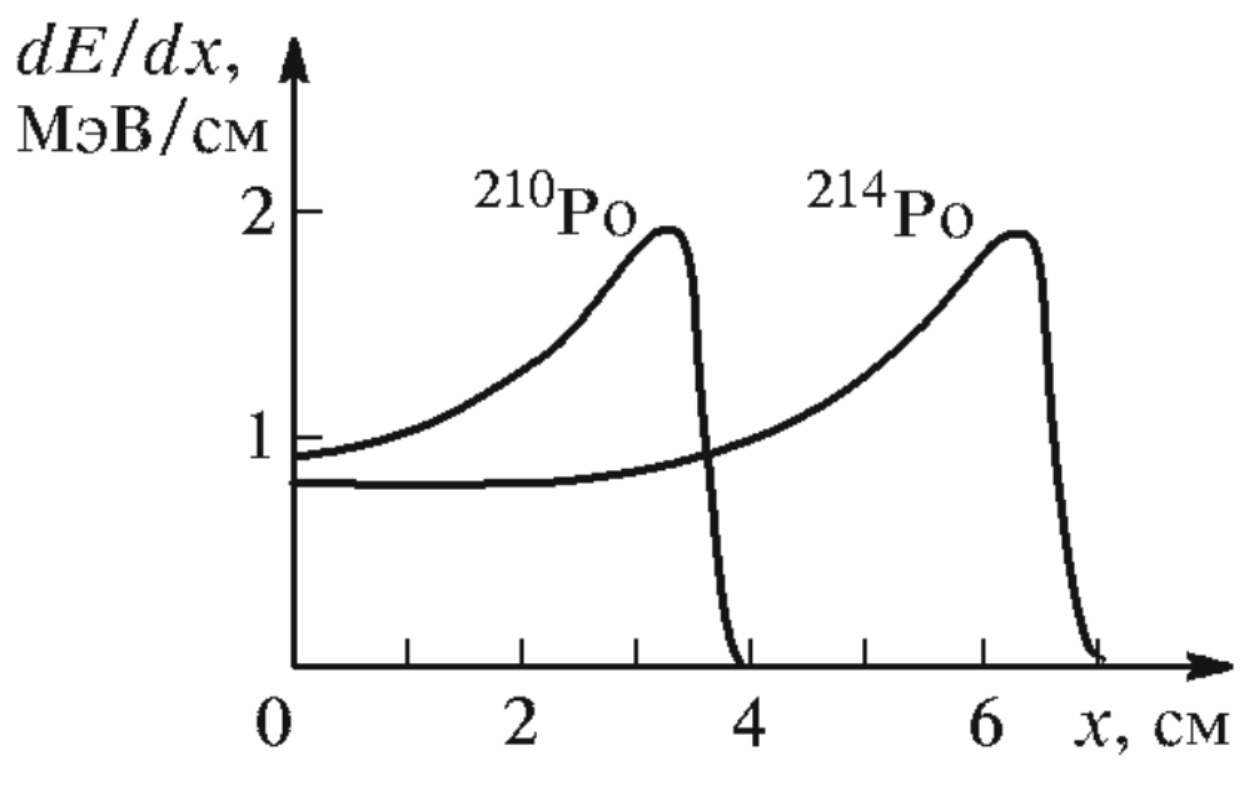
\includegraphics[width=0.6\textwidth]{pic}
        \caption{Кривая Брэгга}
    \end{figure}
	\section{Экспериментальная часть}
	    В этой работе мы исследуем длину пробега альфа-частиц тремя способами:
	    \begin{enumerate}
	        \item С помощью счетчика Гейгера
	        \item С помощью сцинтилляционного счетчика
	        \item С помощью ионизационной камеры
	    \end{enumerate}
	    
	            \begin{figure}[h!]
	            	\centering
	            	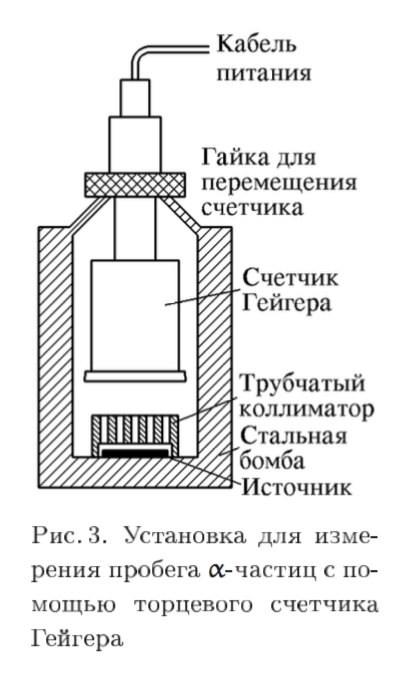
\includegraphics[width=0.3\textwidth]{1}
	            \end{figure}
	                    \begin{figure}[h!]
	                    	\centering
	                    	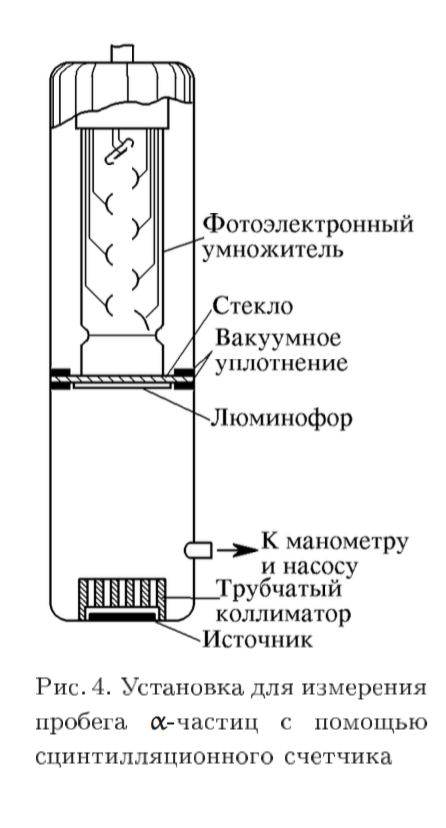
\includegraphics[width=0.3\textwidth]{2}
	                    \end{figure}
	                            \begin{figure}[h!]
	                            	\centering
	                            	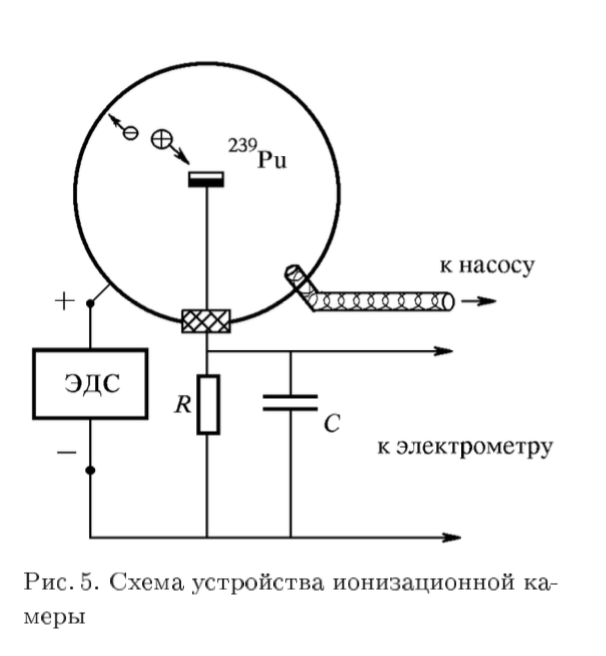
\includegraphics[width=0.3\textwidth]{3}
	                            \end{figure}
	                            
	    
	\section{Экспериментальные данные}
		С помощью счётчика Гейгера исследуем скорость счёта альфа-частиц в зависимости от расстояния до счётчика. Построим график и определим среднюю и экстраполированную длину пробега.
		\begin{figure}[h!]
        \centering
        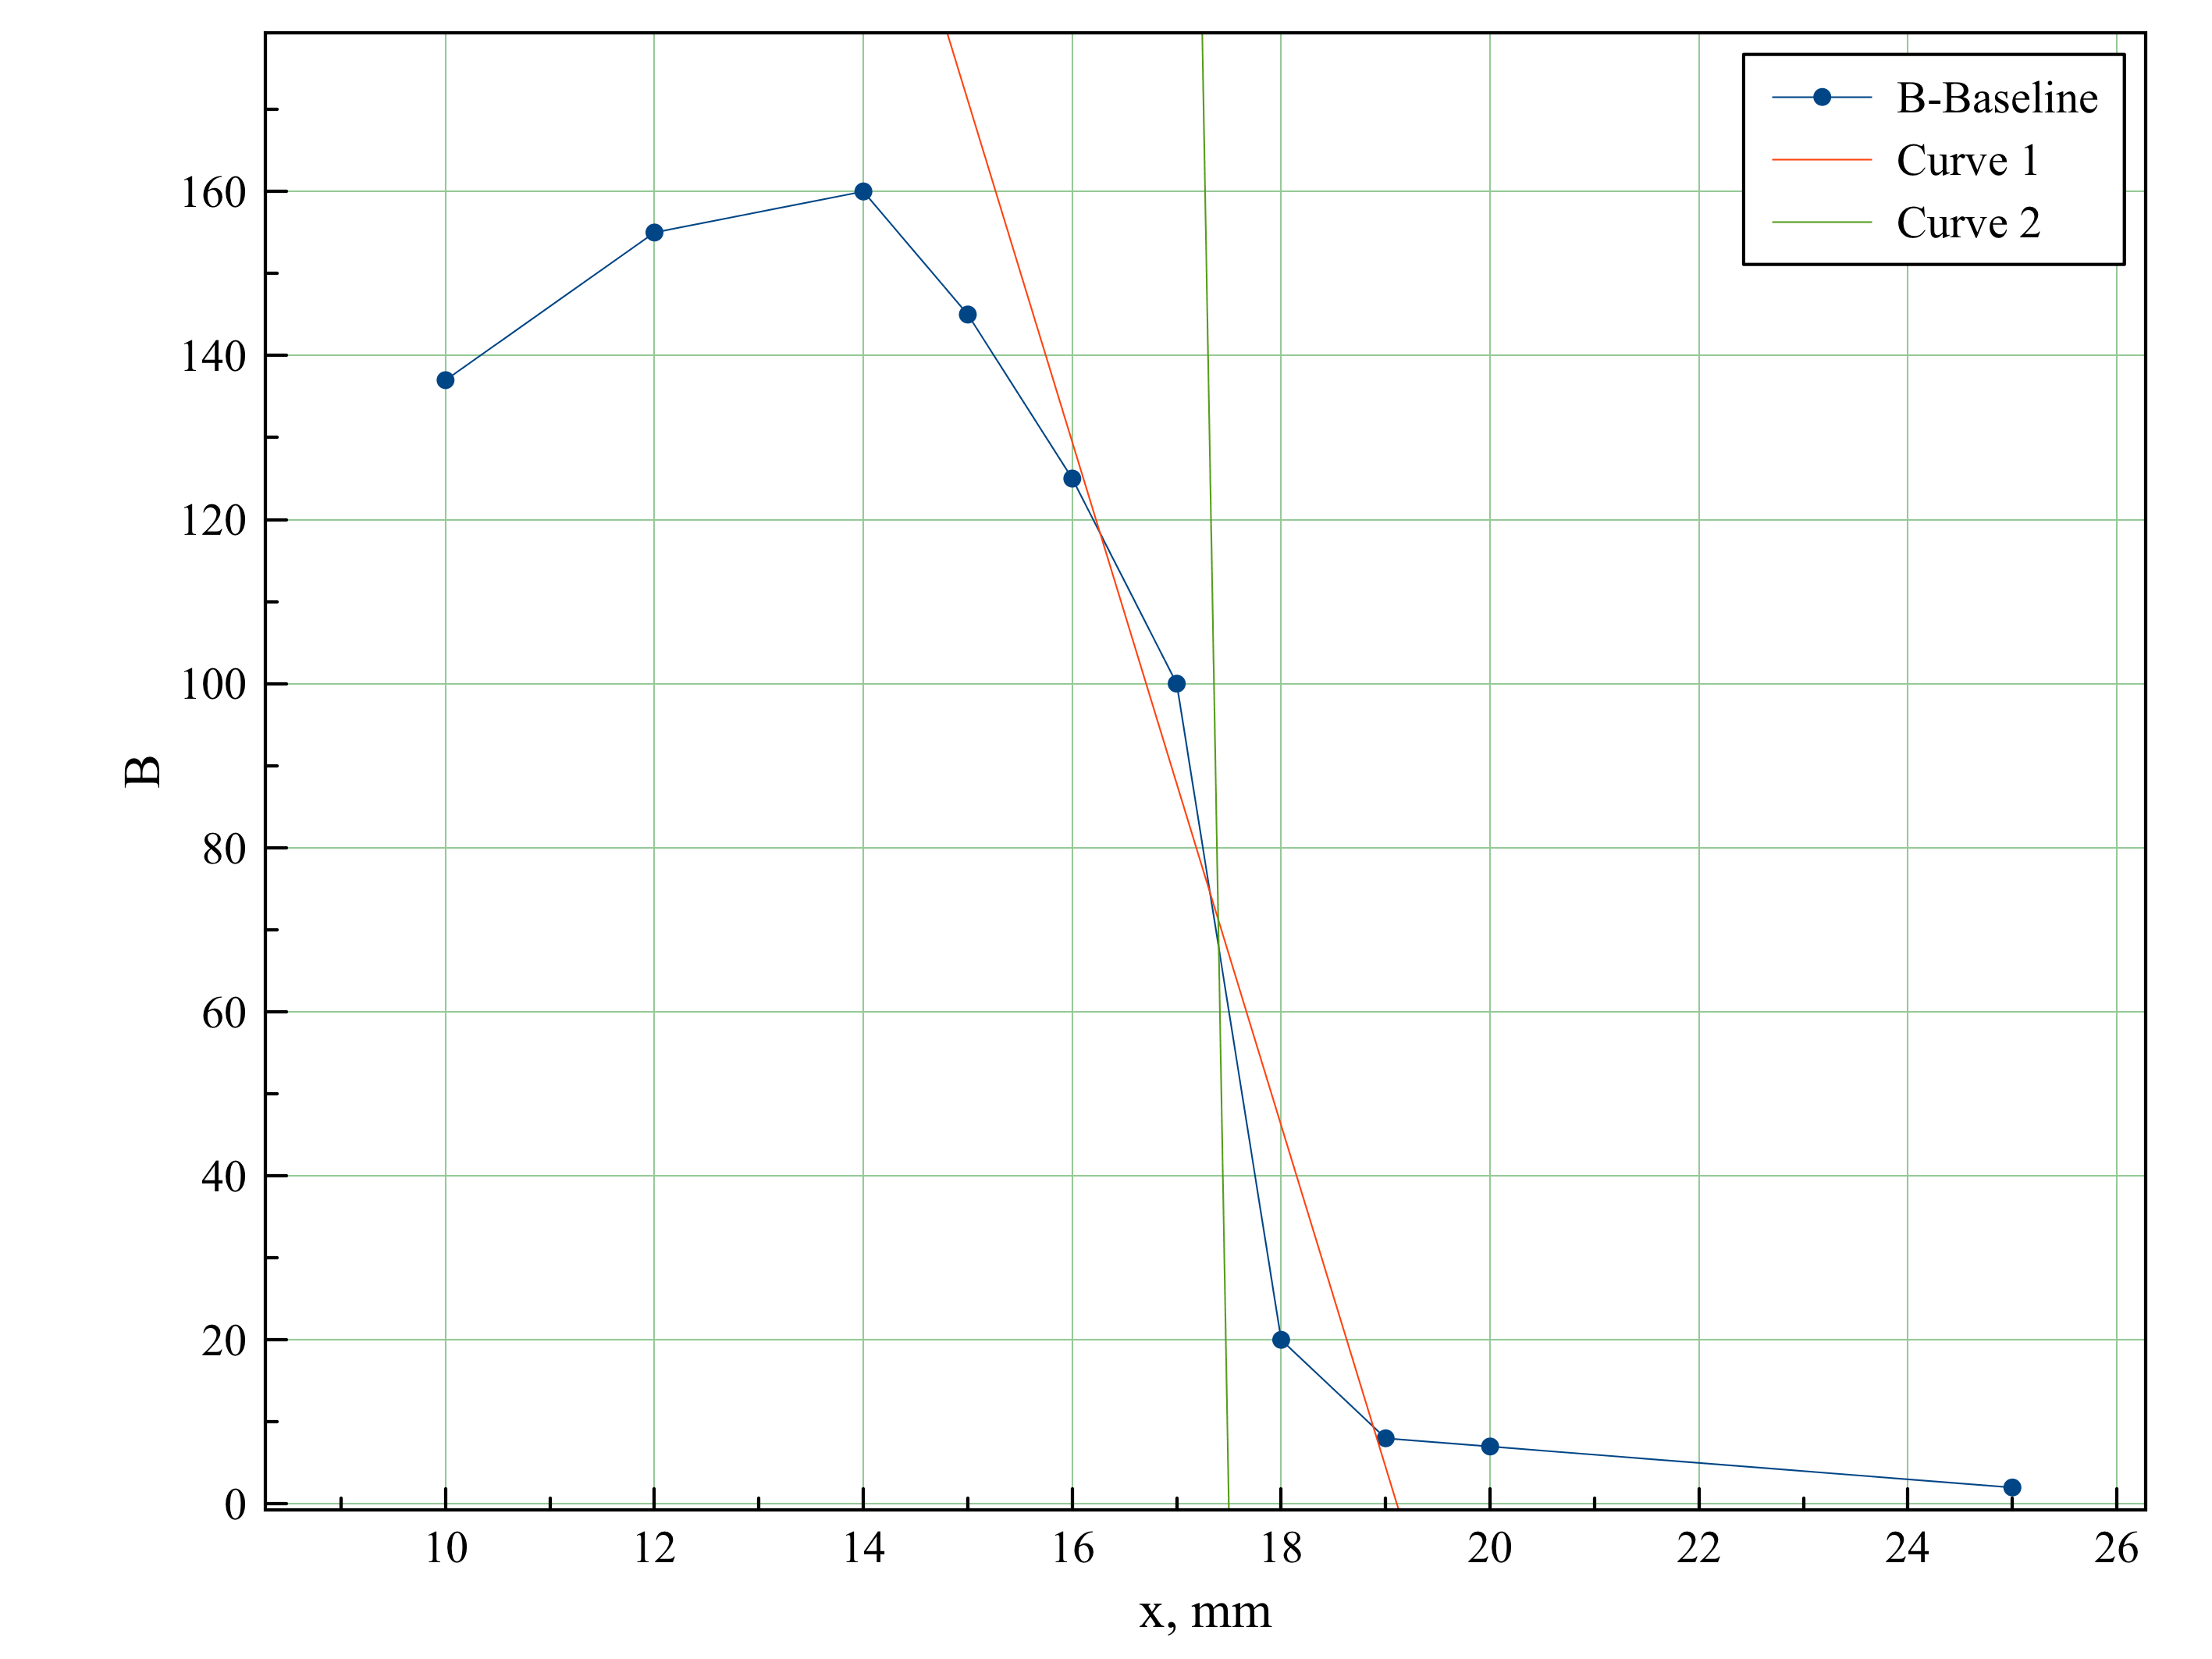
\includegraphics[width=0.8\textwidth]{geig}
        \caption{Зависимость количества счётов от расстояния}
    \end{figure}
    
    Отсюда получим экстраполированную длину $\alpha$-частиц: $R = 19 ~mm$. Средняя длина пробега равна $R = 17,5 ~mm$.
    Рассчитаем энергию: $E = 3.33 MeV$ (из формулы $R=0.32E^{3/2}$)
    
        Повторим исследование с помощью ионизационной камеры. Построим график зависимости тока от давления в камере:
        \pagebreak
        \begin{figure}[h!]
        \centering
        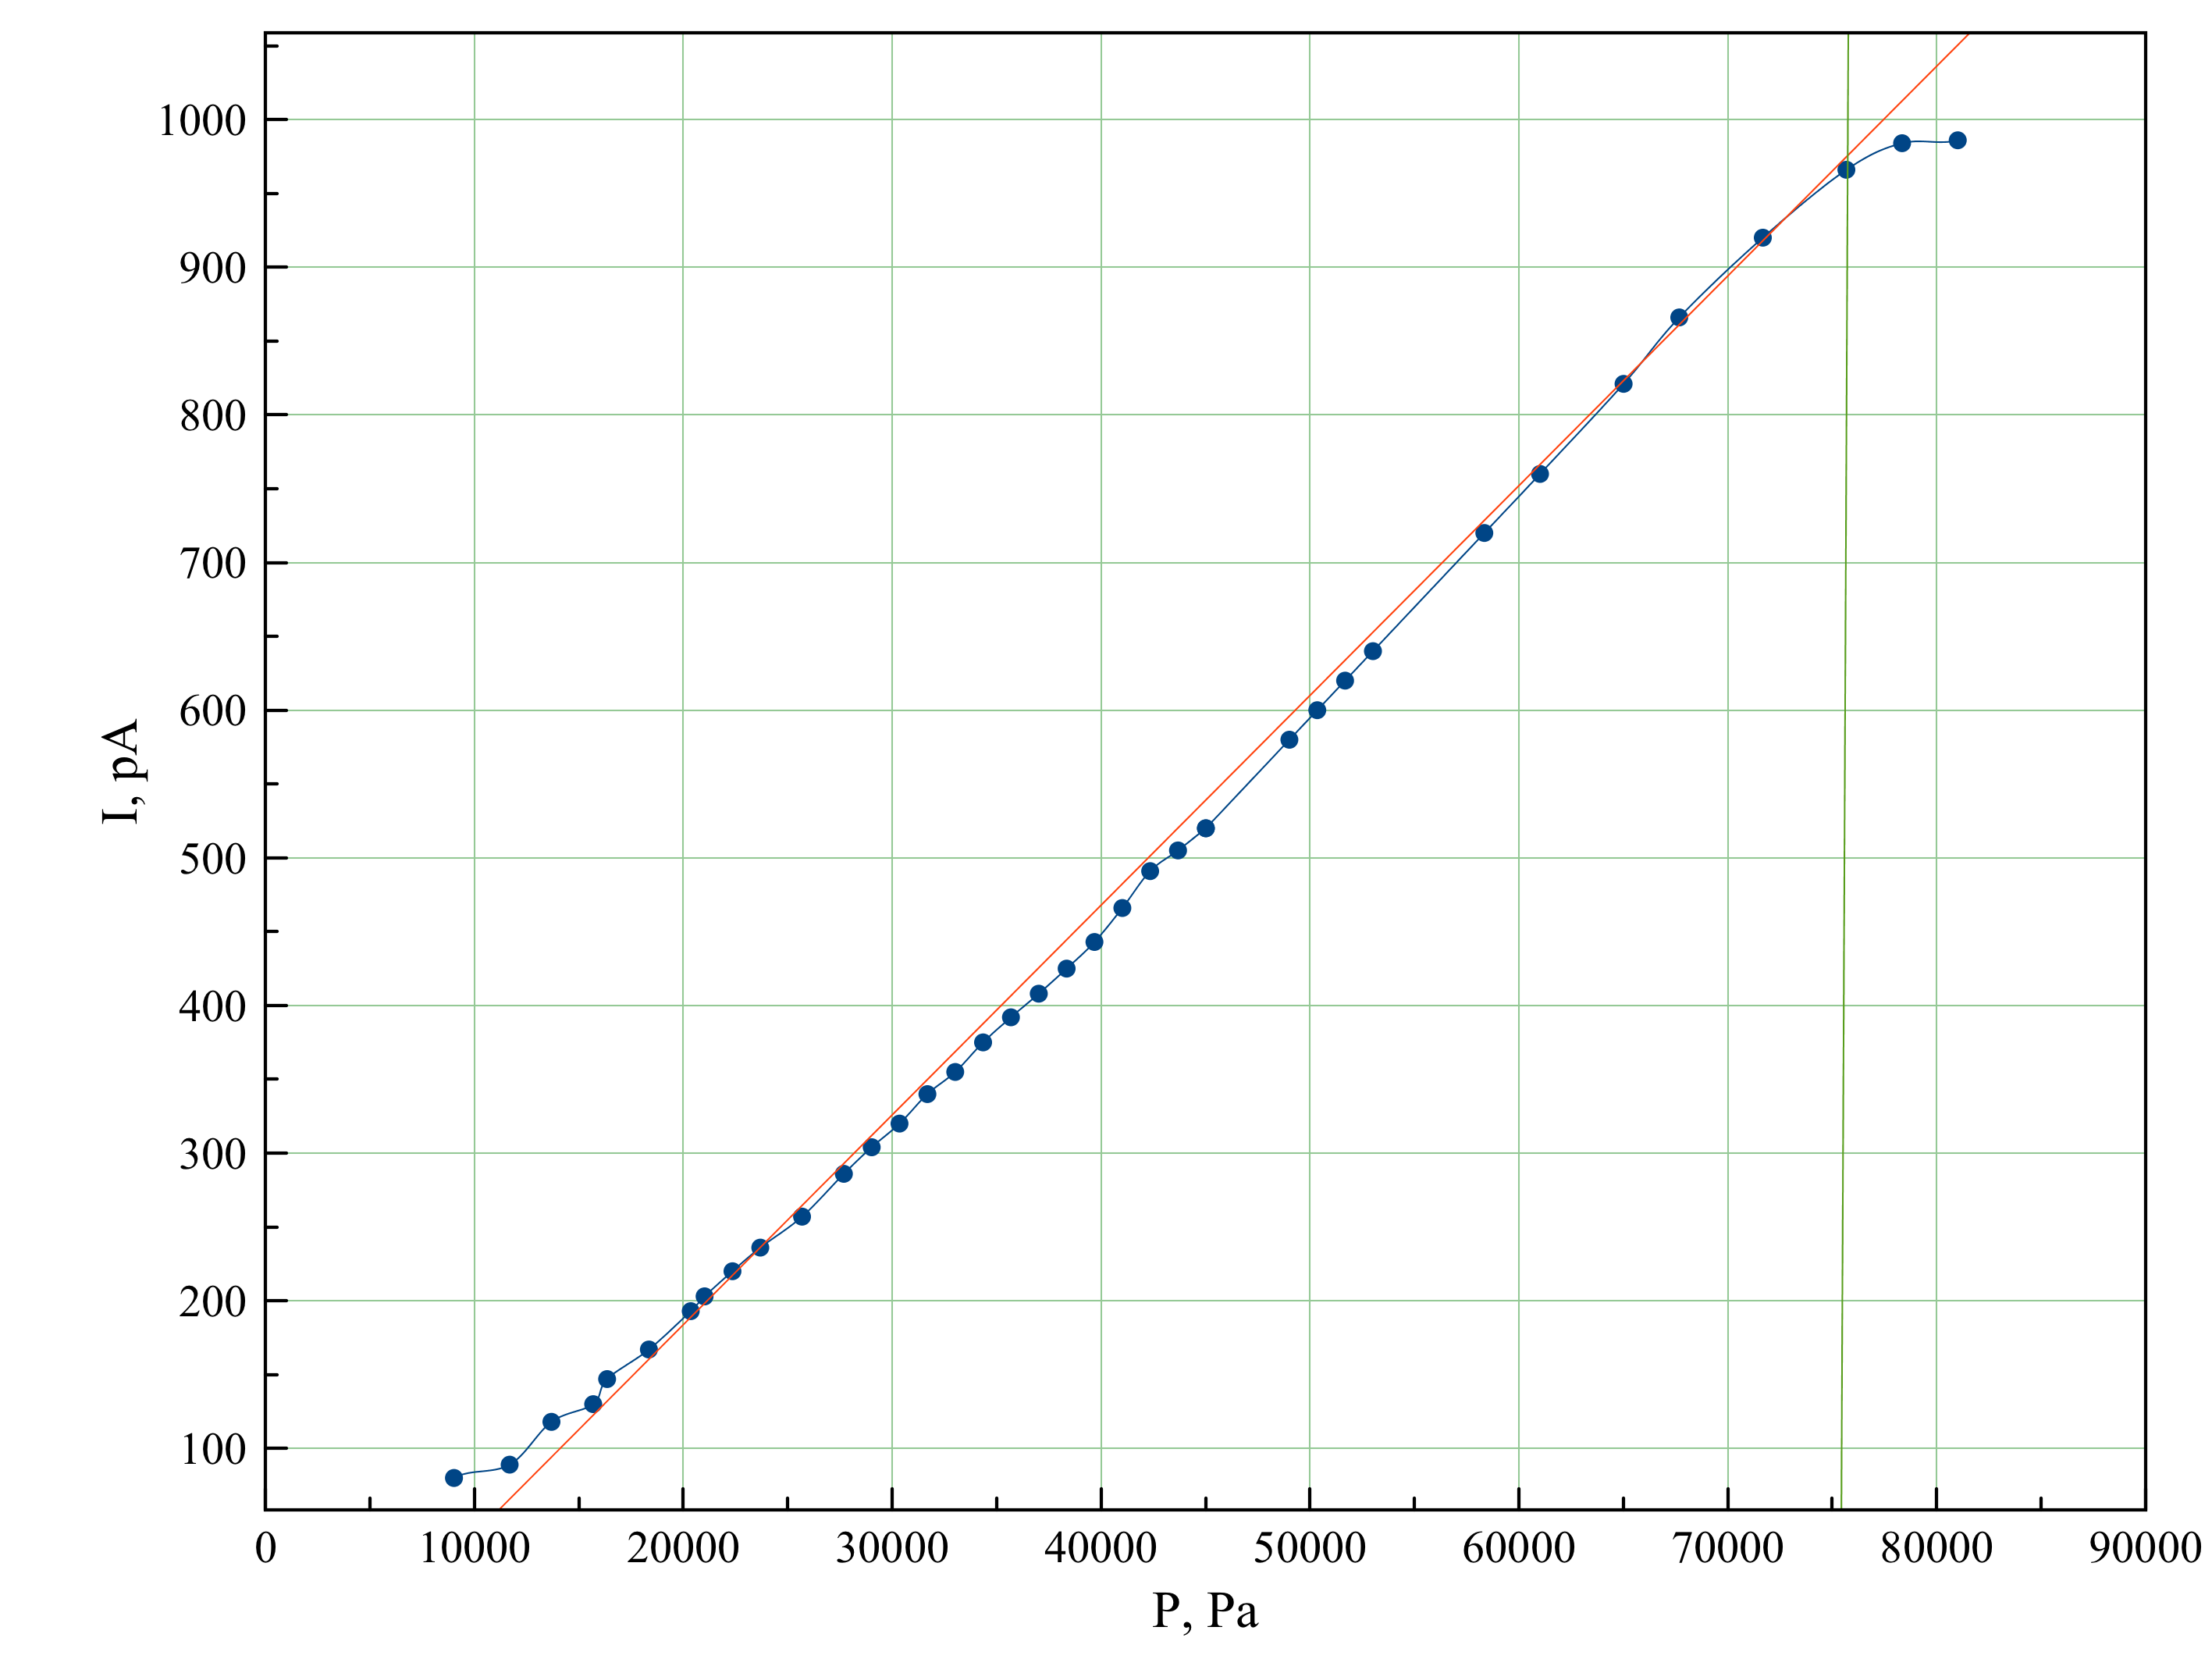
\includegraphics[width=0.8\textwidth]{nasos}
        \caption{Зависимость тока от давления }
    \end{figure}
    
    Эктраполированная длина пробега $R = 38.8 mm$. Отсюда энергия частиц равна $E = 5.28 MeV$
    
    Исследуем длину пробега с помощью сцинтилляционного детектора:
    \begin{figure}[h!]
        \centering
        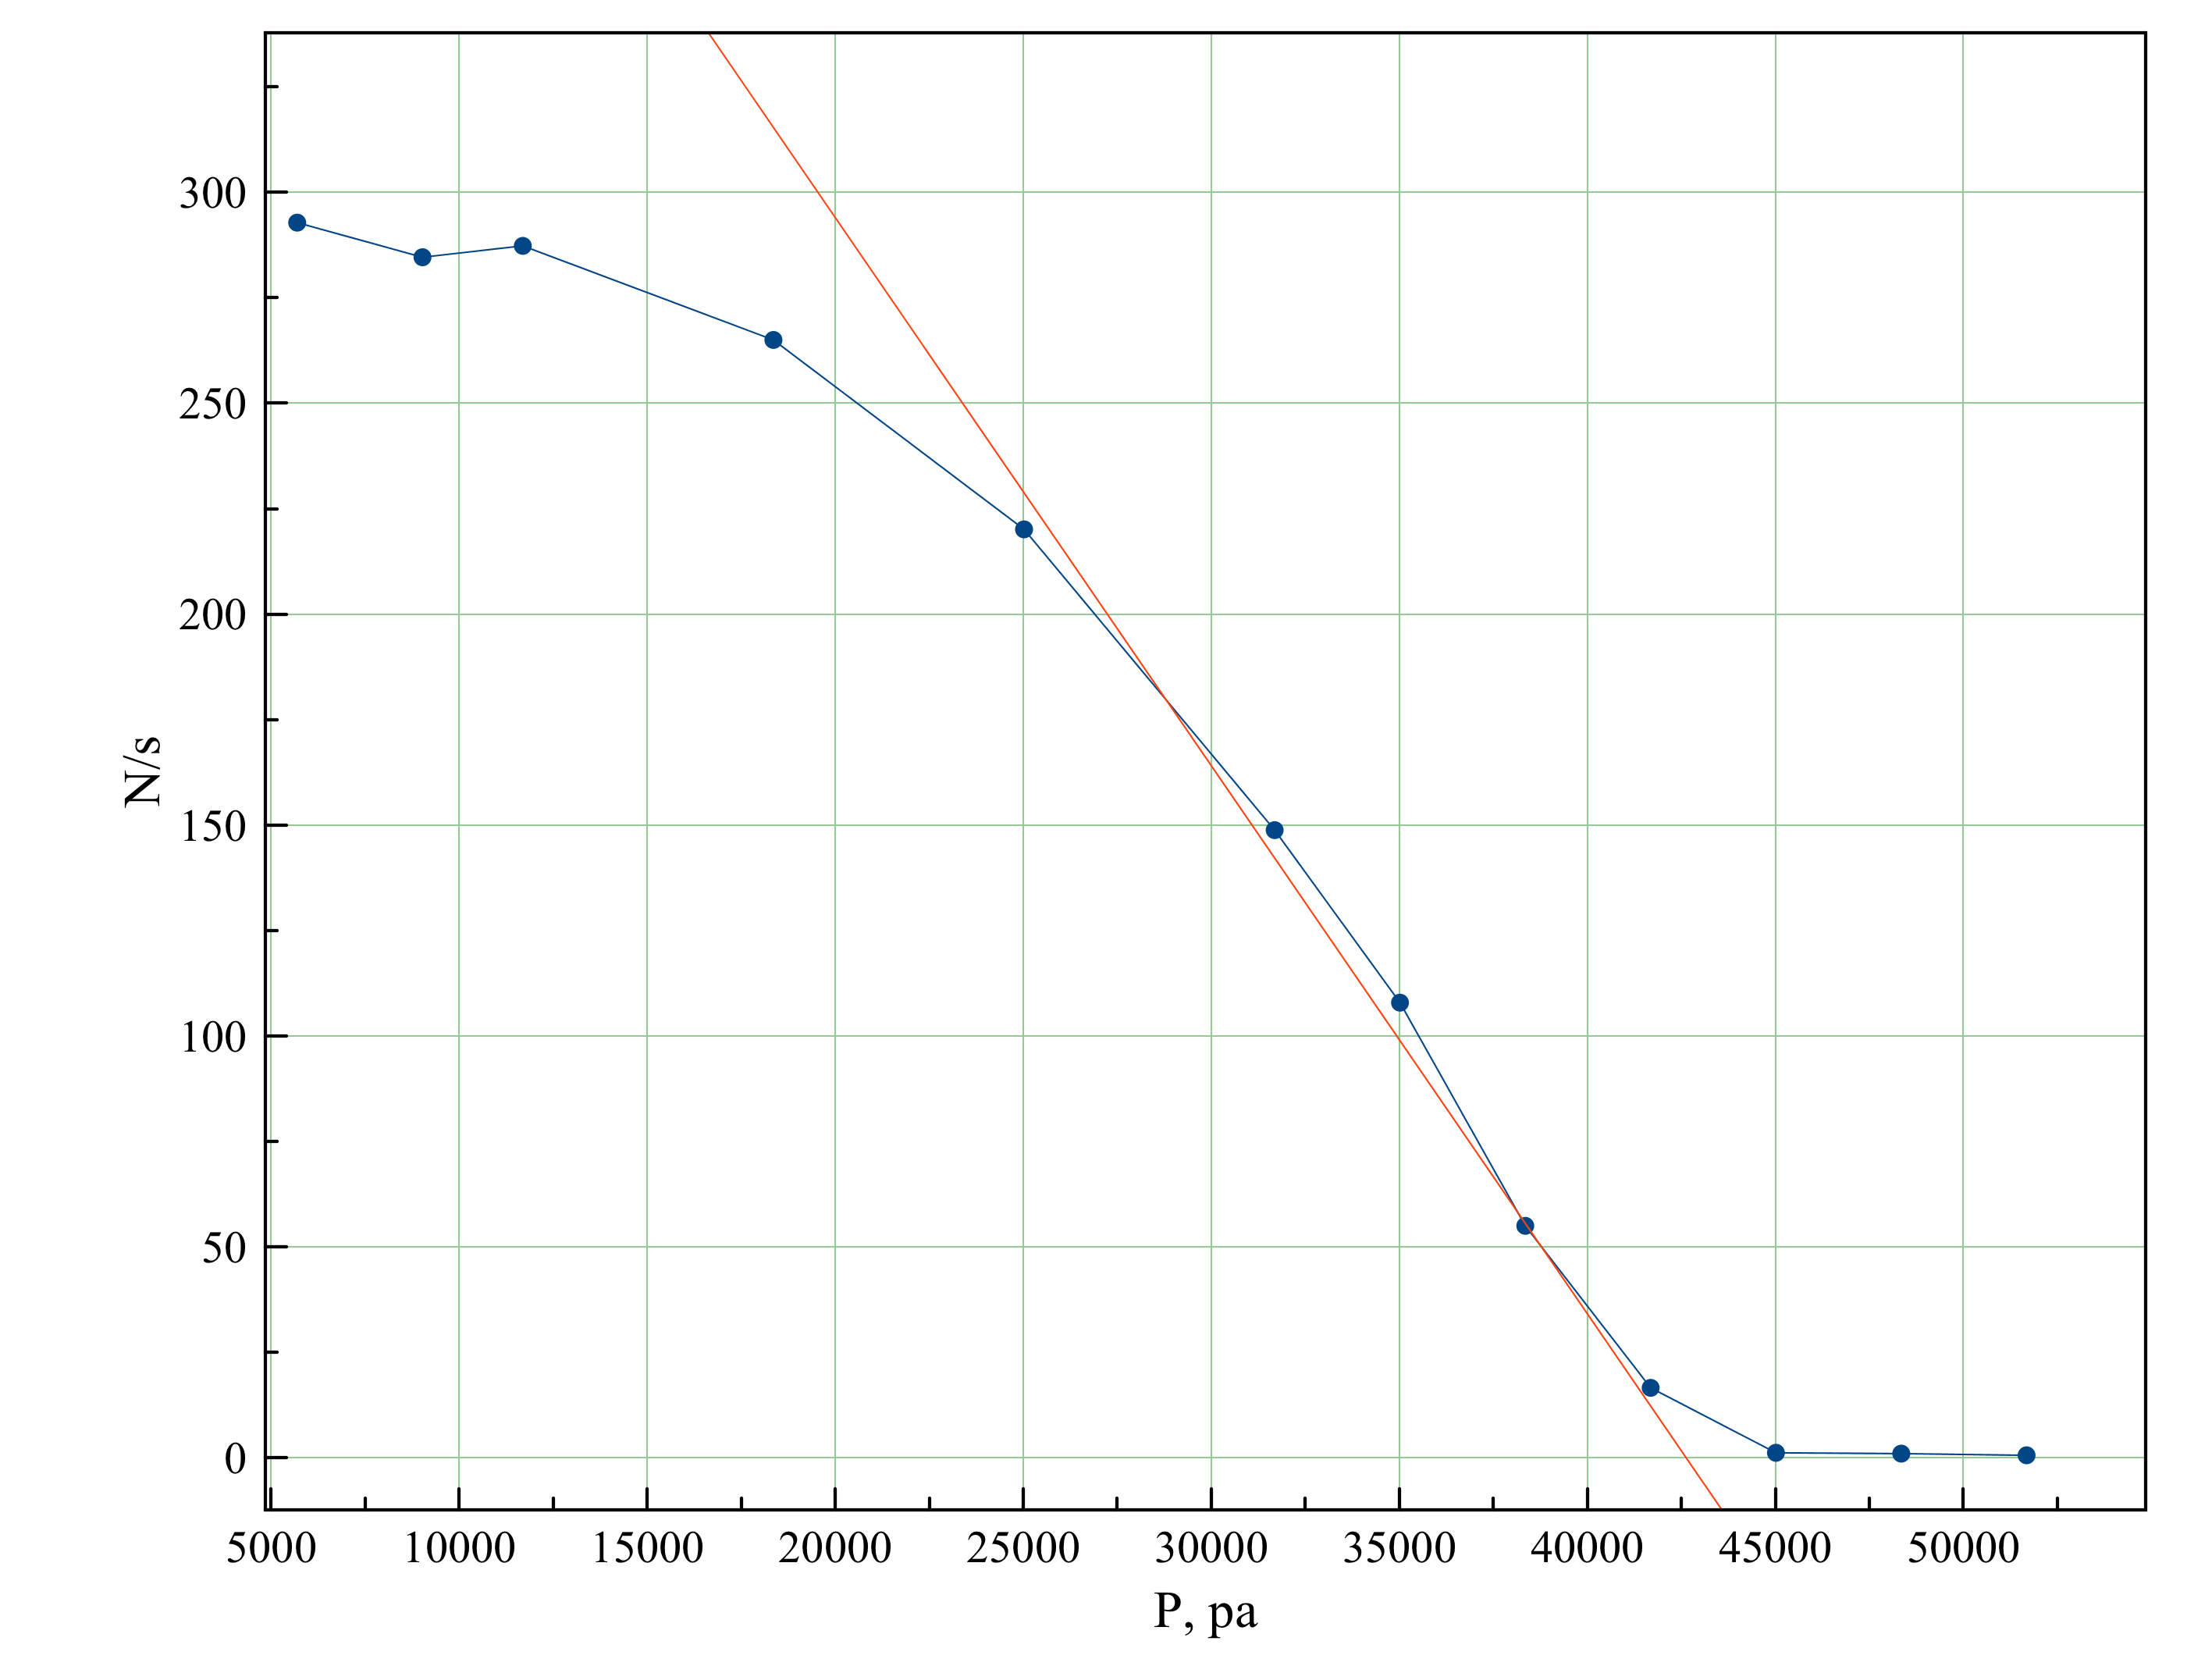
\includegraphics[width=0.8\textwidth]{truba}
        \caption{Сцинтилляционный счетчик}
    \end{figure}
    
    Эктраполированная длина пробега $R = 38.2 mm$. Энергия частиц равна $E = 5.22 MeV$
    


\pagebreak
    
	\section{Вывод}
    Измерили пробег альфа-частиц в воздухе с помощью счетчика Гейгера, сцинтилляционного счетчика и ионизационной камеры. По этим данным определили энергию альфа-частиц. Энергия $\alpha$-частиц при распаде $^{239}Pu$ можно считать приблизительно равной  5.15 МэВ. Наиболее точным методом оказалась ионизационная камера, наименее точным --- счётчик Гейгера.
\end{document}


